\documentclass{article}
\usepackage{tikz}
\usetikzlibrary{positioning, calc}
\usepackage{amsmath, amssymb}
\usepackage[margin=0.9in]{geometry}
\usepackage{caption}
\captionsetup{font=small, labelfont=bf}

% ==========================================
% GLOBAL TIKZ STYLES AND MACROS
% ==========================================
\tikzset{
    base node/.style={circle, draw, minimum size=1.0cm, font=\sffamily\bfseries\large, thick},
    derived node/.style={circle, draw, minimum size=0.85cm, inner sep=1pt, font=\sffamily\small\bfseries, thick, fill=white},
    edge label/.style={font=\sffamily\small, fill=white, inner sep=1.5pt},
}

% Colors used consistently for voltage 0 / 1 / 2 throughout the document
\colorlet{volt0}{blue}
\colorlet{volt1}{red}
\colorlet{volt2}{green!55!black}

% Draw the 3 base nodes on a larger equilateral triangle
\newcommand{\drawbase}{
    \node[base node] (u) at (0,0) {\( u \)};
    \node[base node] (v) at (4,0) {\( v \)};
    \node[base node] (w) at (2,3.46) {\( w \)};
}

% Step 1: invisible coordinates for the 3x3 grid, spaced out to reduce edge crowding.
% Edges are drawn against these bare coordinates; the visible node circles are drawn
% afterwards (see \drawfibernodes) so that edges never paint over a node's fill or label.
\newcommand{\drawfibers}{
    \foreach \name/\x in {u/0, v/4.5, w/9} {
        \coordinate (\name0) at (\x, 6);
        \coordinate (\name1) at (\x, 3);
        \coordinate (\name2) at (\x, 0);
    }
}

% Step 2: the visible fiber labels and node circles, drawn last so they sit on top of
% every edge.
\newcommand{\drawfibernodes}{
    \foreach \name/\x in {u/0, v/4.5, w/9} {
        \node[font=\sffamily\bfseries, text=gray] at (\x, 7.3) {Fiber \name};
        \node[derived node, draw=volt0, text=volt0] at (\name0) {\(\name,0\)};
        \node[derived node, draw=volt1, text=volt1] at (\name1) {\(\name,1\)};
        \node[derived node, draw=volt2, text=volt2] at (\name2) {\(\name,2\)};
    }
}

% Draw the undirected intra-fiber loops (lifts of base loops form a C_3 in each fiber)
\newcommand{\drawderivedloops}{
    \foreach \name in {u, v, w} {
        \draw[-, thick, darkgray, opacity=0.85] (\name0) to (\name1);
        \draw[-, thick, darkgray, opacity=0.85] (\name1) to (\name2);
        \draw[-, thick, darkgray, opacity=0.85, bend right=40] (\name0) to (\name2);
    }
}

% Macro to draw lifts of a single undirected edge between fibers
\newcommand{\drawlift}[3]{
    % #1 = source fiber, #2 = target fiber, #3 = voltage (relative to src -> dst orientation)
    \ifnum#3=0
        \draw[-, thick, volt0, opacity=0.7] (#10) to (#20);
        \draw[-, thick, volt0, opacity=0.7] (#11) to (#21);
        \draw[-, thick, volt0, opacity=0.7] (#12) to (#22);
    \fi
    \ifnum#3=1
        \draw[-, thick, volt1, opacity=0.6] (#10) to (#21);
        \draw[-, thick, volt1, opacity=0.6] (#11) to (#22);
        \draw[-, thick, volt1, opacity=0.6] (#12) to (#20);
    \fi
    \ifnum#3=2
        \draw[-, thick, volt2, opacity=0.6] (#10) to (#22);
        \draw[-, thick, volt2, opacity=0.6] (#11) to (#20);
        \draw[-, thick, volt2, opacity=0.6] (#12) to (#21);
    \fi
}

% One-line color legend, reused above every derived graph
\newcommand{\voltagelegend}{%
    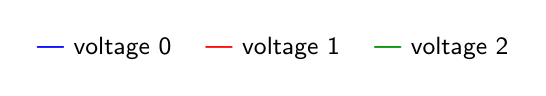
\begin{tikzpicture}[baseline]
        \node[font=\sffamily\small] at (0,0) {\textcolor{volt0}{\textbf{---}} voltage 0 \quad
                                              \textcolor{volt1}{\textbf{---}} voltage 1 \quad
                                              \textcolor{volt2}{\textbf{---}} voltage 2};
    \end{tikzpicture}%
}

\begin{document}

\begin{center}
    {\LARGE\sffamily\bfseries Voltage Graphs on \(\mathbb{Z}_3\) and Their Derived Covers}\\[4pt]
    {\small\sffamily In each pair below, the left figure is the base graph \( \Gamma \) with edges/loops
    labeled by elements of \(\mathbb{Z}_3\); the right figure is the derived (covering) graph \( \Gamma^\lambda \),
    with three fibers of three vertices each. Edge colors in the derived graphs indicate voltage: \\[2pt]
    \voltagelegend}
\end{center}

\vspace{0.3cm}

% ==========================================
% CASE 1: Only 1- and 2- loops
% ==========================================
\begin{center}
    \centering
    \vspace*{1cm}
    {\normalsize\sffamily\bfseries Case 1 of 4: Only loops labeled \(1,2\)}\\[6pt]
    \begin{minipage}[c]{0.435\textwidth}
        \centering
        \begin{tikzpicture}[scale=1.0]
            \drawbase
            \path[-, thick]
            (u) edge [loop left, looseness=8] node[edge label] {\( 1,2 \)} (u)
            (v) edge [loop right, looseness=8] node[edge label] {\( 1,2 \)} (v)
            (w) edge [loop above, looseness=8] node[edge label] {\( 1,2 \)} (w);
        \end{tikzpicture}
        \captionof{figure}{Base \( \Gamma \): undirected loops}
    \end{minipage}\hfill
    \begin{minipage}[c]{0.515\textwidth}
        \centering
        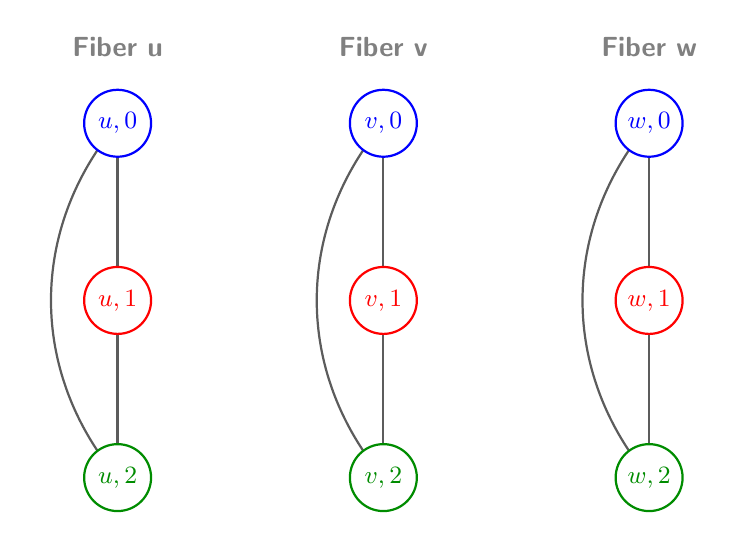
\begin{tikzpicture}[scale=0.75]
            \drawfibers
            \drawderivedloops
            \drawfibernodes
        \end{tikzpicture}
        \captionof{figure}{Derived \( \Gamma^\lambda \): undirected 3-cycles}
    \end{minipage}
\end{center}

\newpage

% ==========================================
% CASE 2: 1- and 2- cycles along with loops
% ==========================================
\begin{center}
    \centering
    \vspace*{1cm}
    {\normalsize\sffamily\bfseries Case 2 of 4: Loops plus a \(1\)-voltage triangle}\\[6pt]
    \begin{minipage}[c]{0.435\textwidth}
        \centering
        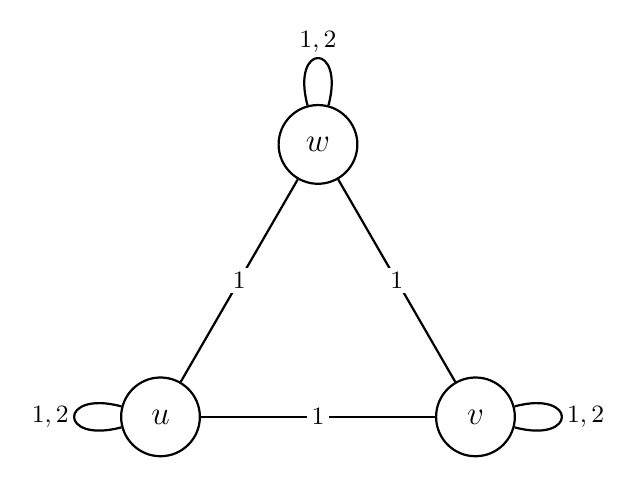
\begin{tikzpicture}[scale=1.0]
            \drawbase
            \path[-, thick]
            (u) edge [loop left, looseness=8] node[edge label] {\( 1,2 \)} (u)
            (v) edge [loop right, looseness=8] node[edge label] {\( 1,2 \)} (v)
            (w) edge [loop above, looseness=8] node[edge label] {\( 1,2 \)} (w)
            (u) edge node[edge label] {\( 1 \)} (v)
            (v) edge node[edge label] {\( 1 \)} (w)
            (w) edge node[edge label] {\( 1 \)} (u);
        \end{tikzpicture}
        \captionof{figure}{Base \( \Gamma \): undirected triangle \& loops}
    \end{minipage}\hfill
    \begin{minipage}[c]{0.515\textwidth}
        \centering
        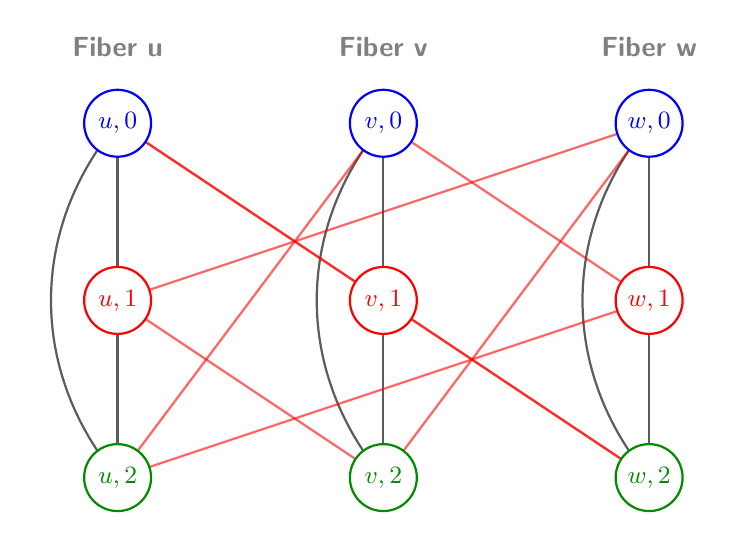
\begin{tikzpicture}[scale=0.75]
            \drawfibers
            \drawderivedloops
            \drawlift{u}{v}{1}
            \drawlift{v}{w}{1}
            \drawlift{w}{u}{1}
            \drawfibernodes
        \end{tikzpicture}
        \captionof{figure}{Derived \( \Gamma^\lambda \) (exactly 18 undirected edges)}
    \end{minipage}
\end{center}

\newpage

% ==========================================
% CASE 3: All 1's and all 2's
% ==========================================
\begin{center}
    \centering
    \vspace*{1cm}
    {\normalsize\sffamily\bfseries Case 3 of 4: Loops plus \(1\)- and \(2\)-voltage triangle edges}\\[6pt]
    \begin{minipage}[c]{0.435\textwidth}
        \centering
        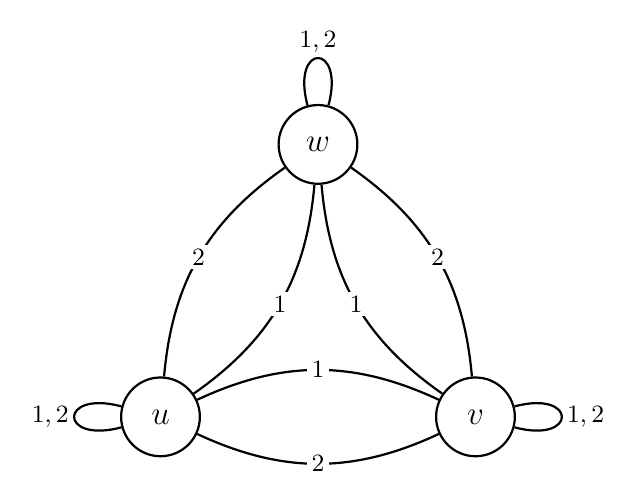
\begin{tikzpicture}[scale=1.0]
            \drawbase
            \path[-, thick]
            (u) edge [loop left, looseness=8] node[edge label] {\( 1,2 \)} (u)
            (v) edge [loop right, looseness=8] node[edge label] {\( 1,2 \)} (v)
            (w) edge [loop above, looseness=8] node[edge label] {\( 1,2 \)} (w)
            (u) edge [bend left=25] node[edge label] {\( 1 \)} (v)
            (u) edge [bend right=25] node[edge label] {\( 2 \)} (v)
            (v) edge [bend left=25] node[edge label] {\( 1 \)} (w)
            (v) edge [bend right=25] node[edge label] {\( 2 \)} (w)
            (w) edge [bend left=25] node[edge label] {\( 1 \)} (u)
            (w) edge [bend right=25] node[edge label] {\( 2 \)} (u);
        \end{tikzpicture}
        \captionof{figure}{Base \( \Gamma \): undirected multigraph}
    \end{minipage}\hfill
    \begin{minipage}[c]{0.515\textwidth}
        \centering
        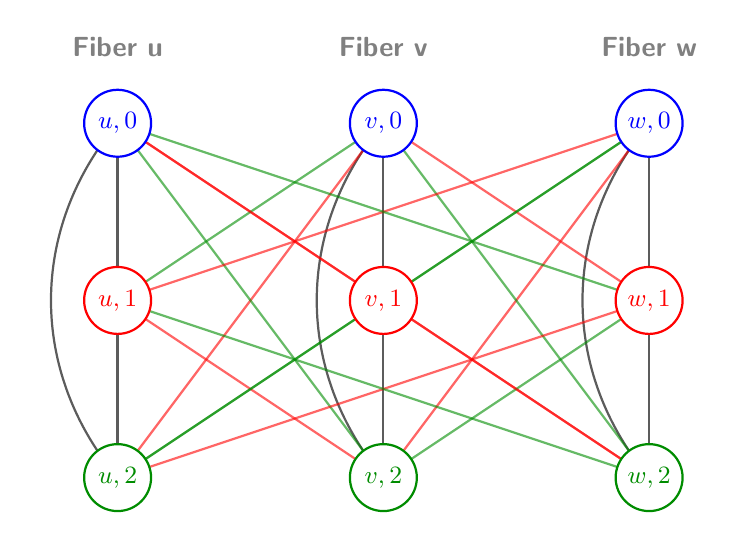
\begin{tikzpicture}[scale=0.75]
            \drawfibers
            \drawderivedloops
            \foreach \src/\dst in {u/v, v/w, w/u} {
                \drawlift{\src}{\dst}{1}
                \drawlift{\src}{\dst}{2}
            }
            \drawfibernodes
        \end{tikzpicture}
        \captionof{figure}{Derived \( \Gamma^\lambda \) (partial \(K_{3,3}\) between fibers)}
    \end{minipage}
\end{center}

\newpage

% ==========================================
% CASE 4: Everything except 0-loops
% ==========================================
\begin{center}
    \centering
    \vspace*{1cm}
    {\normalsize\sffamily\bfseries Case 4 of 4: Loops plus \(0\)-, \(1\)-, and \(2\)-voltage triangle edges}\\[6pt]
    \begin{minipage}[c]{0.435\textwidth}
        \centering
        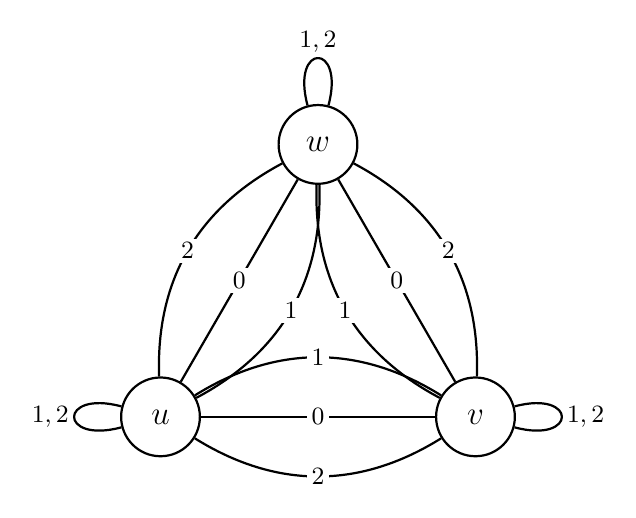
\begin{tikzpicture}[scale=1.0]
            \drawbase
            \path[-, thick]
            (u) edge [loop left, looseness=8] node[edge label] {\( 1,2 \)} (u)
            (v) edge [loop right, looseness=8] node[edge label] {\( 1,2 \)} (v)
            (w) edge [loop above, looseness=8] node[edge label] {\( 1,2 \)} (w)
            (u) edge [bend left=32] node[edge label] {\( 1 \)} (v)
            (u) edge node[edge label] {\( 0 \)} (v)
            (u) edge [bend right=32] node[edge label] {\( 2 \)} (v)
            (v) edge [bend left=32] node[edge label] {\( 1 \)} (w)
            (v) edge node[edge label] {\( 0 \)} (w)
            (v) edge [bend right=32] node[edge label] {\( 2 \)} (w)
            (w) edge [bend left=32] node[edge label] {\( 1 \)} (u)
            (w) edge node[edge label] {\( 0 \)} (u)
            (w) edge [bend right=32] node[edge label] {\( 2 \)} (u);
        \end{tikzpicture}
        \captionof{figure}{Base \( \Gamma \): full undirected multigraph}
    \end{minipage}\hfill
    \begin{minipage}[c]{0.515\textwidth}
        \centering
        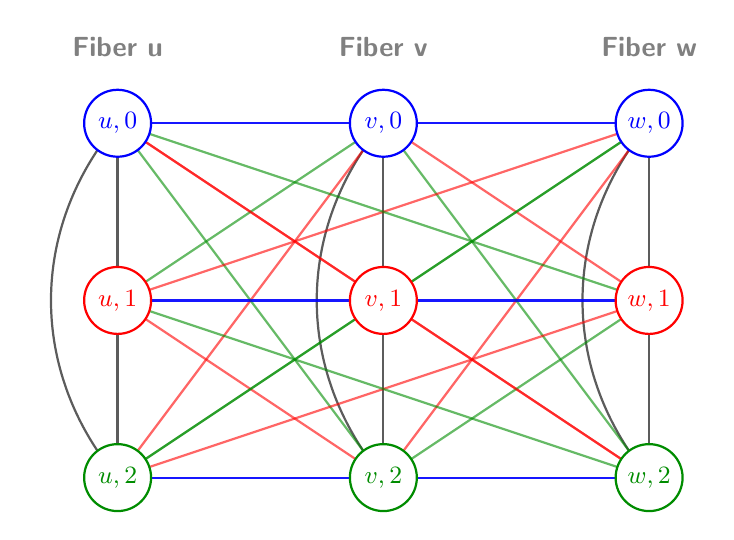
\begin{tikzpicture}[scale=0.75]
            \drawfibers
            \drawderivedloops
            \foreach \src/\dst in {u/v, v/w, w/u} {
                \drawlift{\src}{\dst}{0}
                \drawlift{\src}{\dst}{1}
                \drawlift{\src}{\dst}{2}
            }
            \drawfibernodes
        \end{tikzpicture}
        \captionof{figure}{Derived \( \Gamma^\lambda \) (perfect \(K_{3,3}\) between all fibers)}
    \end{minipage}
\end{center}

\end{document}
